\documentclass[11pt,a4paper]{report}

\usepackage[utf8]{inputenc}
\usepackage{graphics}
\usepackage{amsmath}

\usepackage[hidelinks]{hyperref}
\usepackage{url} 

\usepackage{pdfpages}
\usepackage{pdflscape}
\usepackage{pythonhighlight}
\usepackage{amssymb}
\usepackage{braket}

\usepackage[resetlabels,labeled]{multibib}

\newcounter{counter}[section]
\renewcommand{\thecounter}{\thechapter.\arabic{counter}}

\newenvironment{definition}[1]{\bigskip\refstepcounter{counter}\noindent\textbf{Definition \thecounter } \emph{#1} \par\nopagebreak\noindent \begin{itshape}}{\end{itshape}\bigskip}

\newenvironment{example}[1]{\bigskip\refstepcounter{counter}\noindent\textbf{Example \thecounter} \emph{#1} \par\nopagebreak}{\bigskip}

\newenvironment{notation}{\bigskip\refstepcounter{counter}\noindent\textbf{Notation \thecounter~}\nopagebreak \begin{itshape}}{\end{itshape}\bigskip}

\newenvironment{theorem}{\bigskip\refstepcounter{counter}\noindent\textbf{Theorem \thecounter }\nopagebreak \begin{itshape}}{\end{itshape}\medskip}

\newenvironment{lemma}{\bigskip\refstepcounter{counter}\noindent\textbf{Lemma \thecounter }\nopagebreak \begin{itshape}}{\end{itshape}\bigskip}

\newenvironment{remark}{\bigskip\refstepcounter{counter}\noindent\textbf{Remark \thecounter~ }\nopagebreak \begin{itshape}}{\end{itshape}\bigskip}

\definecolor{gray}{rgb}{0.4,0.4,0.4}
\definecolor{graybright}{rgb}{0.5,0.5,0.5}
\definecolor{darkblue}{rgb}{0.0,0.0,0.6}
\definecolor{cyan}{rgb}{0.0,0.6,0.6}

\lstset{
  basicstyle=\ttfamily,
  columns=fullflexible,
  showstringspaces=false,
  commentstyle=\color{gray}\upshape
}

\lstdefinelanguage{XML}
{
  morestring=[b]",
  morestring=[s]{>}{<},
  morecomment=[s]{<?}{?>},
  stringstyle=\color{black},
  identifierstyle=\color{darkblue},
  keywordstyle=\color{cyan},
  morekeywords={xmlns,version,type}% list your attributes here
}

\lstdefinelanguage{LBS}
{
  stringstyle=\color{black},
  keywordstyle=\textbf,
  morekeywords={spec, new, comp, inside}% list your attributes here
}

\begin{document}

%---------preamble generated from fithesis template
\includepdf[pages={2}]{preamble/pre.pdf}

\pagestyle{plain}
\pagenumbering{roman}

~\vfill

\section*{Acknowledgements}
I would like to thank ...


\newpage
%~\vfill
\section*{Abstract}
My abstract is as follow

\newpage
\section*{Keywords}
Keyword1, keyword2, keyword3...

\tableofcontents
\newpage

\setcounter{page}{0}
\pagenumbering{arabic}

%--------------------------------------------------------

\chapter{Introduction} \label{chap:intro}

Modelling complex systems in systems biology has to be conducted at several levels of abstraction that reflect well the known information~\cite{Kitano}. At every level, the system has to be described rigorously in a formal language that allows to avoid
misunderstanding and ambiguous interpretations. The more complex the system is, the harder it is to describe it rigorously while not losing human-readability and compactness of the description at the same time.

Traditional approaches used to describe biochemical systems are: a \emph{chemistry approach} employing ``mechanical'' descriptions by chemical reactions or a \emph{mathematical approach} using ordinary differential equations or other mathematical formalisms. An advantage of chemical reactions over mathematical equations is the fact that chemical reactions are composable to some extent, human-readable and well-understood across disciplines while still having an executable semantics. 
Moreover, there are methods automatising the generation of mathematical models from chemical equations.

The problem of both approaches is the \emph{scalability} which is understood at two
different levels: scalability of the model description (avoiding combinatorial explosion at the syntactic level) and scalability of the model execution (avoiding combinatorial explosion at the semantics level). Even when the formulation of a model does not run into syntactic scalability problems, the execution or simulation might be infeasible~\cite{Romers107136}. 

The so-called \emph{computational approach}~\cite{Cardelli,Henzinger} offers scalable model description by abstracting the information about individual model components and interactions. The scalability at the semantics level still remains to be a challenge. A promising computational approach is provided by \emph{rule-based modelling}~\cite{kappa_formal, BNGL} and process-algebraic frameworks~\cite{Cardelli,BioPEPA,BioSPI}. Rule-based models make a natural extension of the mechanical reaction-based models used in chemistry. Instead of operating with \emph{objects}, rule-based frameworks operate with \emph{types} that allow to avoid the combinatorial explosion that occurs when underlying objects are specified directly. The semantics of the model is given in terms of \emph{rules} defined on given types. An important advantage of rule-based approach is that mathematical models can be automatically generated from it. In particular, instead of relying on a single mathematical formalism, different mathematical models can thus be obtained for a given model (e.g., ODEs~\cite{KaDE}, PDEs~\cite{Smoldyn}, chemical master equation or continuous-time Markov chains~\cite{Pauleve2010,sneddon2011efficient}, reaction-diffusion systems~\cite{So2013}, etc.). 

The long-term aim of our research is the development of Comprehensive Modelling Platform~\cite{cs2bio2013,BCS} -- a general modelling framework that combines model building, model analysis, and annotation tasks in a single public site related to a single system. It respects the need for maintaining existing ODE models (which is still a typical scenario in systems biology) but allows to align them with a mechanistic rule-based description that is understandable by biologists, compact in size, and executable in terms of allowing basic analysis tasks ensuring consistency of the description. Such a comprehensive solution allows to support modellers effort in building mathematical models that have clear biochemical meaning and can be
easily integrated. Moreover, mechanistic descriptions can be later used as standalone computational models having all advantages of rule-based modelling. 

To that end, we have pioneered an idea of combining advantages of rule-based modelling with the simplicity of chemical reactions by introducing a rule-based language called \emph{Biochemical Space Language} (BCSL), introduced in~\cite{Ded201627}. It has the following key aspects: \emph{human-readability} -- easy to read, write, and maintain;
\emph{executability} -- formal executable semantics is defined allowing efficient static analysis and consistency checking; \emph{universality} -- principally different cellular processes can be sufficiently combined in a single specification; and \emph{syntactic scalability} -- combinatorial explosion of the description is avoided. However, similarly as in any other rule-based language, the problem of the \emph{model execution scalability} is not covered efficiently.

We propose a scalable approach based on formal methods to analysis of rule-based models. The emphasis is placed on parameter synthesis using a symbolic method and static analysis enabled by unique level of abstraction enabled by rule-based approach. The methods will be demonstrated using BCSL but their applicability should be universal across other rule-based formalisms.

\chapter{Rule-based modelling}
\label{formal}

Generally, a rule-based system is based on \emph{rewriting} of some structured objects called \emph{agents} according to predefined \emph{rules}. The structure defined on the agents enables varying the level of context given in the rules. The less context given, the wider is the domain the rule can be applied to. It is the key feature which supports the conciseness of rule-based approach.

In this chapter, we define a simplified version of rule-based system. The defined rules are based on a simpler objects called \emph{reactions}, which are used for rewriting of of unstructured objects. Then, the rule can be seen as a set of these reactions. \textbf{TBA - has to be improved...}

\begin{definition}{Multiset}
\emph{Multiset} $\mathtt{M}$ is a pair $(\mathcal{A}, \mathtt{m})$ where $\mathcal{A}$ is a set and $ \mathtt{m} : \mathcal{A} \rightarrow \mathbb{N} $ is a function from $\mathcal{A}$ to the set of natural numbers. The set $\mathcal{A}$ is called the \emph{reference set} of elements. For each element $\mathit{a}$ in $\mathcal{A}$ the \emph{multiplicity} (that is, number of occurrences) of $\mathit{a}$ is the number $\mathtt{M}(\mathit{a})$.
\end{definition}

The elements of the multiset are often referenced as \emph{species}. We denote with $\mathbb{M}$ the set of all multisets. With $\Gamma$ we denote the set of all arbitrary rational functions over the domain of species. The notation $\nu(\mathtt{M})$ with $\nu \in \Gamma$ and $\mathtt{M} \in \mathbb{M}$ denotes the evaluation of function $\nu$ to a rational number by substituting each variable $\mathit{a}$ by its corresponding value $\mathtt{M}(\mathit{a})$.

\begin{definition}{Reaction}
A reaction $\omega$ is a triple $(\mathtt{lhs}, \mathtt{rhs}, \nu) \in \mathbb{M} \times \mathbb{M} \times \Gamma$ where $\mathtt{lhs}$ is left-hand side, $\mathtt{rhs}$ is right-hand side, and $\nu$ is a rational rate function.
\end{definition}

Informally, a reaction states how different species interact to change the number of objects of the corresponding species in the state of the system. The state of the system is an unstructured collection (multiset) of copies of each species. By $\Omega$ we denote the set of all reactions.

\begin{definition}{Reaction application}
Let $\omega = (\mathtt{lhs}, \mathtt{rhs}, \nu)$ be a reaction and $\mathtt{M}$ be a multiset. The \emph{reaction application} to the multiset $\mathtt{M}$, written $\omega(\mathtt{M})$, is a pair $(\mathtt{M} - \mathtt{lhs} + \mathtt{rhs}, \nu(\mathtt{M}))$ if $\mathtt{M} - \mathtt{lhs} > 0$; $(\mathtt{M}, 0)$ otherwise.
\end{definition}

Applying a reaction to a state (multiset) means removing from the state the elements that appear in the left-hand side ($\mathtt{lhs}$) of the reaction and adding the elements that appear on the right-hand side ($\mathtt{rhs}$) of the reaction. Additionally, the \emph{rate function} $\nu$ is evaluated in the process and provides reaction rate, i.e. speed at which the reaction happens. In the case when the number of occurrences of some species required by $\mathtt{lhs}$ is not high enough, the application is not possible and the rate is zero. For an example of reaction application, see Figure~\ref{reaction_example}.

\begin{figure}[!h]
	\begin{center}
		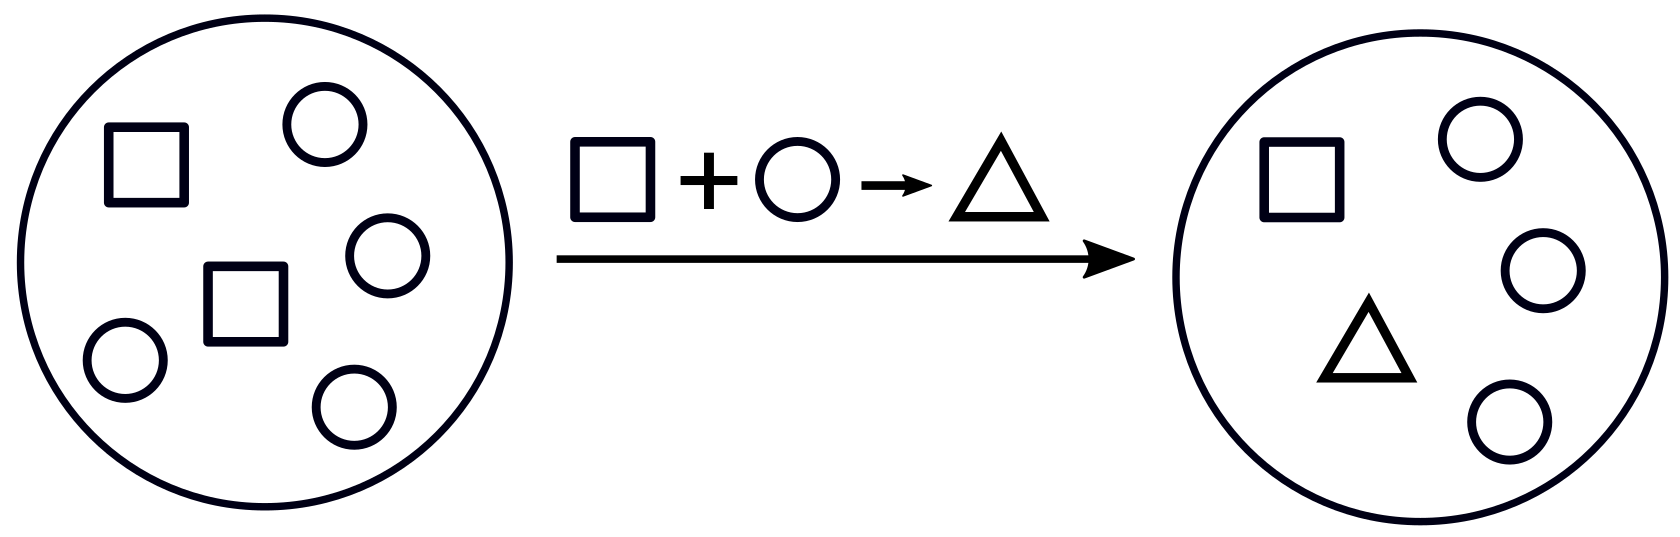
\includegraphics[scale=0.2]{images/reaction.png}
	\end{center}
	\caption{A graphical example of reaction application. In a multiset represented by a big circle we have three kinds of agents -- {\large $\square$}, \raisebox{0.04cm}[0cm]{{$\bigcirc$}} and $\bigtriangleup$. In the reaction $\omega = (\{{\large \square}:1,\hspace{0.1cm} $\raisebox{0.04cm}[0cm]{{$\bigcirc$}}\hspace{0.1cm}$:1\}, \{\bigtriangleup:1\}, \mathtt{2}\times{\large \square}\hspace{0.05cm}\times$\hspace{0.05cm}\raisebox{0.04cm}[0cm]{{$\bigcirc$}}$)$, the agents {\large $\square$} and \raisebox{0.04cm}[0cm]{{$\bigcirc$}} are consumed and a new agent $\bigtriangleup$ is produced. The rate of the reaction is given as a function of molecular counts of both reactants. After substituting the counts to {\large $\square$} $ = \mathtt{2}$ and \raisebox{0.04cm}[0cm]{{$\bigcirc$}} $ = \mathtt{4}$, the evaluation of $\mathtt{2} \times \mathtt{2} \times \mathtt{4}$ gives the rate $\mathtt{16}$.}\label{reaction_example}
\end{figure}

\begin{definition}{Rule}
A rule $\rho \in 2^\Omega$ is defined as a set of reactions. By $\omega \in \rho$ we denote a reaction from the definition base of rule $\rho$.
\end{definition}

A rule is a generalisation of multiple reactions. Instead of a single possible way of application as in the case of reaction, there are multiple outcomes of the application on a given multiset. By $\Sigma$ we denote the set of all rules. A set of rules, which can be viewed as a high-level compact definition of a chemical reaction network, can be used to obtain a conventional model specification.

\begin{definition}{Rule application}
Let $\rho$ be a rule and $\mathtt{M}$ be a multiset. The \emph{rule application} to the multiset $\mathtt{M}$, written $\rho(\mathtt{M})$, is a set $\{ \omega(\mathtt{M}) ~|~ \omega \in \rho \}$ of all reaction applications from the definition base of the rule.
\end{definition}

Given a multiset, applying a rule to it produces a set of \emph{multiset--rate} pairs. This is caused by the fact that all possible reactions represented by the rule can produce a different outcome (some of them cannot be applied due to non-negative number of repetitions requirement in reaction application). An example of rule application is given in Figure~\ref{rule_example}.

\begin{figure}[!h]
	\begin{center}
		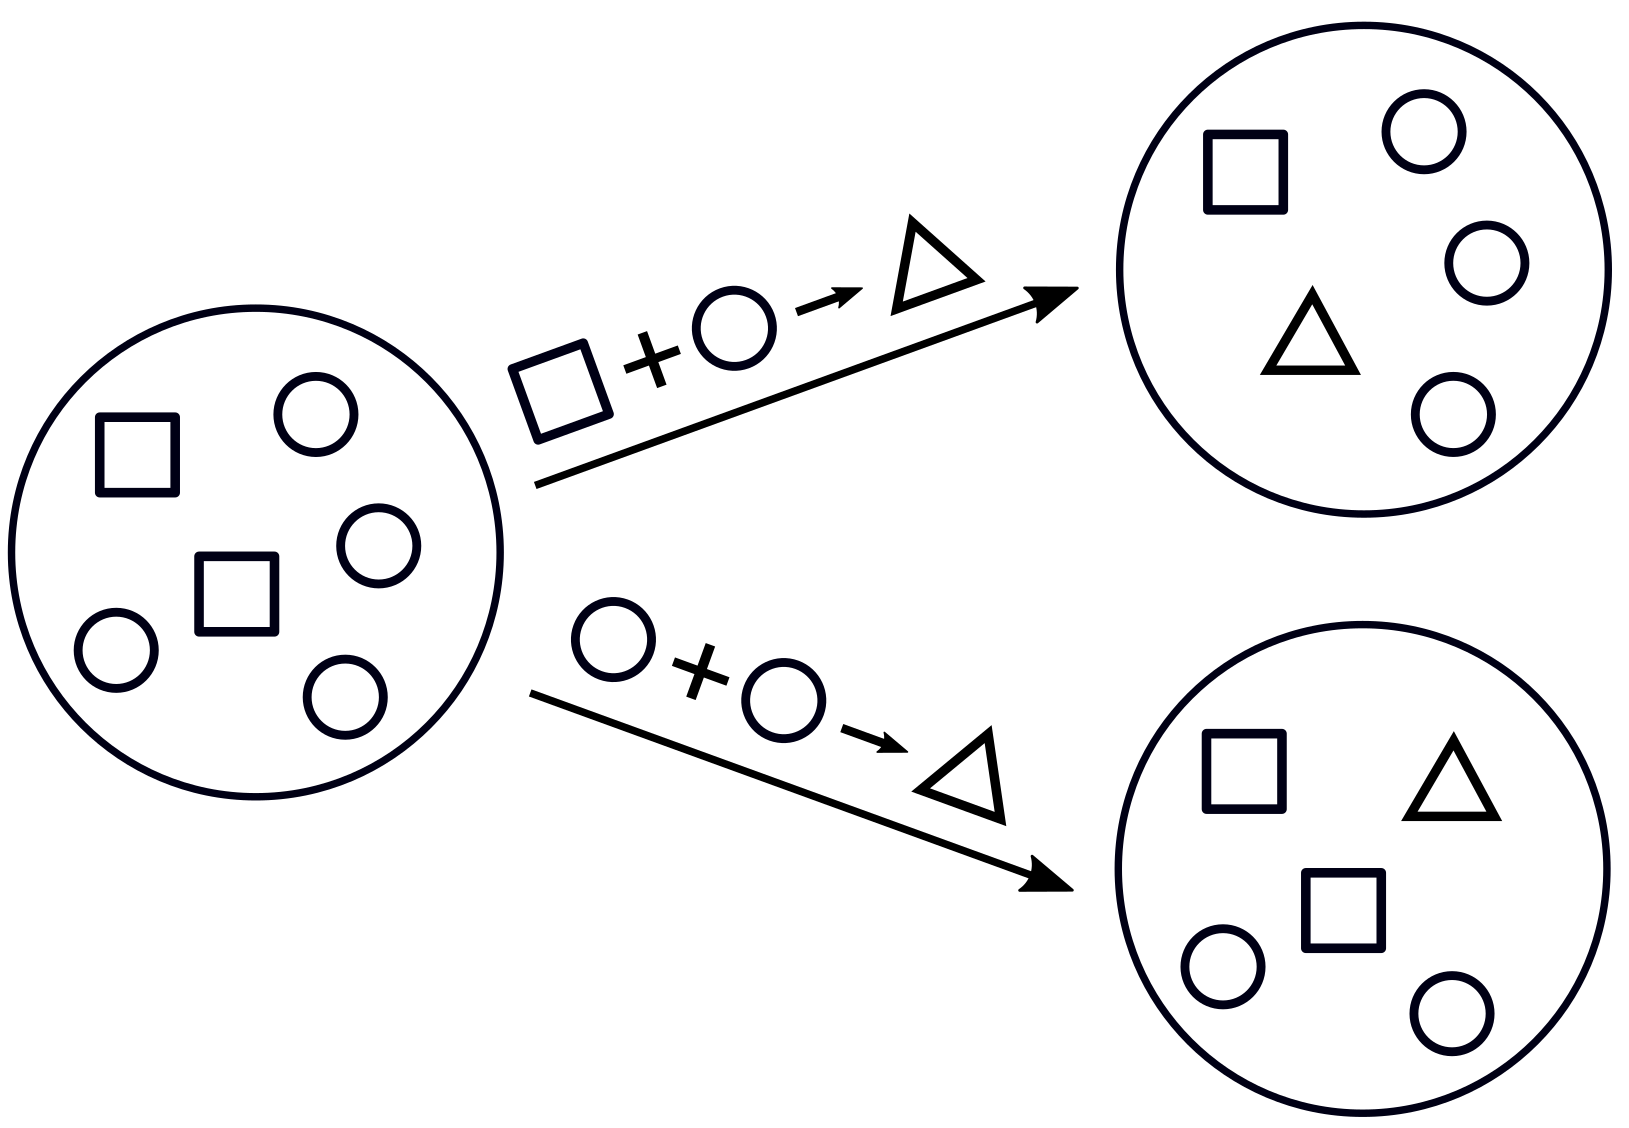
\includegraphics[scale=0.2]{images/rule.png}
	\end{center}
	\caption{A graphical example of reaction application. In a multiset represented by a big circle we have three kinds of agents -- {\large $\square$}, \raisebox{0.04cm}[0cm]{{$\bigcirc$}} and $\bigtriangleup$. Let us have two reactions $\omega_1 = (\{{\large \square}:1,\hspace{0.1cm} $\raisebox{0.04cm}[0cm]{{$\bigcirc$}}\hspace{0.1cm}$:1\}, \{\bigtriangleup:1\}, \mathtt{2}\times{\large \square}\hspace{0.05cm}\times$\hspace{0.05cm}\raisebox{0.04cm}[0cm]{{$\bigcirc$}}$)$ and $\omega_2 = (\{\hspace{0.1cm} $\raisebox{0.04cm}[0cm]{{$\bigcirc$}}\hspace{0.1cm}$:2\}, \{\bigtriangleup:1\}, \mathtt{3}\times$\hspace{0.05cm}\raisebox{0.04cm}[0cm]{{$\bigcirc$}}$^2)$. The rule $\rho = \{ \omega_1, \omega_2 \}$ is given by both reactions. The rule application can therefore produce a different state for each reaction, each created by particular reaction application. The associated rates are $\mathtt{2} \times \mathtt{2} \times \mathtt{4} = \mathtt{16}$ and $\mathtt{3} \times \mathtt{4}^2 = \mathtt{48}$, respectively.}\label{rule_example}
\end{figure}

\begin{definition}{Rule-based model}
A rule-based model $\mu$ is a pair $(\mathcal{R}, \mathtt{M}_0) \in 2^\Sigma \times \mathbb{M}$ where $\mathcal{R}$ is a set of rules and $\mathtt{M}_0$ is an initial state (multiset) of the model.
\end{definition}

A rule-based model is composed from two parts -- the initial state, describing the number of occurrences of individual species in the default situation, and the set of rules which define how the species can interact. The \emph{semantics} of the model is given in terms of rule application, which is transitively applied on the initial state.

A natural extension of the model is \emph{parametrised} rule-based model where rate functions can be enriched by unknown parameters from a known domain (usually integers or rational numbers). It is a typical case in systems biology since the actual values of reaction kinetics are often hard or even impossible to be measured. Then, to evaluate a rate function, a \emph{parametrisation} $p$ from the admissible parameter space has to be given, representing a particular biological scenario.

An important advantage of rule-based approach is that mathematical models can be automatically generated from it. In particular, instead of relying on a single mathematical formalism, different mathematical models can thus be obtained for a given model (e.g., ODEs~\cite{KaDE}, chemical master equation or continuous-time Markov chains~\cite{Pauleve2010,sneddon2011efficient}).

This fact results in multiple possible ways how to analyse and explore the models. For example, one can be interested in bifurcation analysis~\cite{benevs2017discrete} or attractor analysis~\cite{benevs2018fully} in ODEs; robustness analysis in continuous-time Markov chains~\cite{vceska2014robustness}; parameter synthesis in parametric discrete-time Markov chains~\cite{daws2004symbolic} etc. Each of the approaches provides a unique point of view how to see the underlying model and enables ??? 

The most of the mentioned analysis methods are based on \emph{model checking}~\cite{clarke2018model}, an automatic way for checking whether the model meets a given specification. For that, we need a specification language which allows us to express a property dependent on time. A suitable tool is to use a \emph{temporal logic}. Examples of logics which are often used in systems biology are LTL (?), CTL (?), STL (?), or PCTL~\cite{hasson1994logic} and their usage depends on particular mathematical representation of use.

\begin{definition}{Model checking}
Given a rule-based model $\mu = (\mathcal{R}, \mathtt{M}_0)$ and a formula $\phi$, the \emph{problem of model checking} is to decide whether the model $\mu$ satisfies the property $\phi$.
\end{definition}

In the case of unknown parameter values present in the model, we can be interested in finding those parametrisations from the parameter space which satisfy the given property. For that, a method called \emph{parameter synthesis} is used. The basic principle is to search parameter space and identify regions where satisfaction is (not) guaranteed. Often regions where no guarantees are given are produced due to some computational error of used searching method.

\begin{definition}{Parameter synthesis}
Given a parametrised rule-based model $\mu = (\mathcal{R}, \mathtt{M}_0)$ and a formula $\phi$, the \emph{problem of parameter synthesis} is to compute a partitioning of the given parameter space into three disjoint subsets: $\mathsf{TRUE}$ -- the model satisfies the property, $\mathsf{FALSE}$ -- the model does \emph{not} satisfy the property, and $\mathsf{UNKNOWN}$ -- the result is not known.
\end{definition}

Additionally, instead of the binary answer to satisfaction of a property, a measure of how much the property is preserved in the given parametrisation can be useful. This measure is called \emph{local robustness} $D^{\mu}_{\phi}(p)$ and states how much the property $\phi$ is preserved in parametrisation $p$ of model $\mu$.

\begin{definition}{Robustness analysis}
The \emph{problem of global robustness} of a model $\mu$ is defined as 

$$ R^{\mu}_{\phi, P} = \int_{P} \psi(p) D^{\mu}_{\phi}(p) dp $$

where $\phi$ is the property of the system under scrutiny, $P$ is the parametrisation space, $\psi(p)$ is the probability of the parametrisation $p$, and $D^{\mu}_{\phi}(p)$ is the local robustness.
\end{definition}

The global robustness~\cite{kitano2007towards} defines a measure of how the given property is preserved globally in the entire model with respect to the parameter space.

\chapter{State of the Art} \label{chap:state}

\section{Rule-based languages}
\label{rule_based_languages}

There are several rule-based languages dedicated for modelling of the biological systems. Each of them uses different features and abstractions. In this chapter, we will highlight the key features of some of the representatives and describe analysis established for them. It is important to note that generally, they can be always formulated in terms defined in Chapter~\ref{formal}.

A specificity of individual languages resides in the level of abstraction they use and the way how they handle the encoding of a rule such that they avoid the explicit reaction representation. The implicit representation they use includes both syntactic and semantic level, providing a direct apparatus of rules execution.

\subsection{Kappa language}
\label{kappa}

The Kappa language~\cite{kappa_formal} was primary developed for the modelling of protein interactions. The key structures used in the language are \emph{agents} with \emph{binding sites}, which allow formation of \emph{bonds} between the agents. Each binding site must be unique with at most one bond. Each site can occur in one of several pre-defined states.

The Kappa \emph{rules} are changing properties of the agents. Particularly, the rule might add, delete, or change a bond or a state of one or multiple agents at once. The rules are patterns with two sides where each of them is a sequence of agents delimited by a comma. The introduction of sites allows to group multiple reactions to a single rule by omitting the context which is not relevant. This is a typical way how rule-based languages encode reactions to rules and it ensures conciseness of description. Example of a rule is in Figure~\ref{kappa-rule}.

\begin{figure}[!h]
\begin{center}
\begin{tabular}{c l}
(a) & A(bsa$\sim$\{ u, p \}) ; B(bsb$\sim$\{ a, i \}) \\
(b) & A(bsa), B(bsb$\sim$a) $\rightarrow$ A(bsa!1), B(bsb$\sim$a!1) \\
\end{tabular}
\end{center}
\caption{Example of a Kappa rule. (a) Definition of associated agents. There are allowed two agents, A and B, both with a binding site which might occur in two possible states. (b) The rule itself. It defines a creation of bond on the sites of agents A and B such that site of agent B must be in an active state. Note the context with no importance for the interaction is omitted, encoding multiple possible reactions.}\label{kappa-rule}
\end{figure}

The general problem present in the Kappa language is too detailed description. For biological systems, it might be often difficult to deal with all the bonds, especially in cases when we do not need such details.

\subsection{BioNetGen Language}
\label{bngl}

The BioNetGen Language (BNGL) \cite{BNGL} is similar to the Kappa language, but there are several differences. The basic idea of the language is to use molecules to describe the building blocks of a biological system such as proteins, genes, and metabolites respectively. Each molecule has a number of sites with associated internal states that are used to represent the status of post-translational modifications or bindings with other molecules. The rules describe the interactions among molecules including associa­tions, dissociations, modifications to the internal state of a site
as well as the production or consumption of molecular species. Rules also provide rate laws for transformations resulting from molecular interactions. Patterns are used to identify a set of molecules that share the same internal states. The rule can be specified using patterns such that it defines not a single reaction but a potentially large class of reactions, all involving a common transformation parametrised by the  same rate law.

BNGL rule typically represent molecular interactions and the consequences of these interactions. An example of a rule is given in Figure~\ref{bngl-rule}. Software tools have been developed to construct, visualize, simulate, and analyse BNGL models~\cite{wenskovitch2014mosbie,harris2016bionetgen,xu2011rulebender,sneddon2011efficient}.

\begin{figure}[!h]
\begin{center}
\begin{tabular}{c l}
(a) & A(bsa$\sim$u$\sim$p) \\
  & B(bsb$\sim$a$\sim$i) \\
(b) & A(bsa) + B(bsb$\sim$a) $\rightarrow$ A(bsa!1).B(bsb$\sim$a!1) \\
\end{tabular}
\end{center}
\caption{Example of a BNGL rule. (a) Definition of associated agents. There are allowed two agents, A and B, both with a binding site which might occur in two possible states. (b) The rule itself. Note that the agents A and B must first create \emph{reaction complex} denoted by `+' (i.e., they must be close to each other) and then they create \emph{complex of agents} denoted by `.' (i.e., they are physically connected).}\label{bngl-rule}
\end{figure}

\subsection{PySB}

The PySB language~\cite{Lopez646} is an open-source programming framework written in Python that allows concepts and methodologies from contemporary software engineering to be applied to the construction of transparent, extensible and reusable biological  models. It is implemented as a package in the Python programming language. 

The definition of the models directly in the code allows the usage of the full syntax of Python, what significantly increases the expression power of PySB. Its widespread use in the computational biology community, support for object-oriented and functional programming, and rich ecosystem of mathematical and scientific libraries makes it an excellent choice of programming language for this purpose. On the other hand, the increased expressive power make the models harder to analyse.

The core of the language is defined by translating to BNGL. PySB is closely integrated with Python numerical tools for simulation and parameter estimation and graphical tools that enable plotting of model trajectories and topologies. The main advantage of the language is that it can be used to decompose models into reusable macros that can be independently tested, and the used to generate composite models. An example of a rule is given in Figure~\ref{pysb_rule}.

\begin{figure}[!h]
\begin{center}
\begin{python}
# Declare the monomers
Monomer('L', ['s'])
Monomer('R', ['s'])

# Declare the binding rule
Rule(L(s=None) + R(s=None) <> L(s=1) % R(s=1), kf, kr)
\end{python}
\end{center}
\caption{Example of a PySB rule. The rule describes creation of a bond between agents $\mathtt{R}$ and $\mathtt{L}$.}\label{PySB-rule}\label{pysb_rule}
\end{figure}

\subsection{Chromar}

The Chromar language~\cite{honorato2017chromar} allows to define attributes for agents and range them over pre-defined domains. The qualitative semantics are given by rule match on multisets composed of these agents producing a reaction. It is followed by standard application of the reaction (in the manner of multiset operations). The language is very useful when creating a model where we need to create new distinct objects and control population of these objects.

Embedding this language into the functional programming language Haskell increases its expressive power while making the ability of some analysis more expensive. Moreover, a user needs to understand Haskell (at least its basics) in order to use Chromar.

It is important to highlight a feature which the stochastic semantics of this language offers. Compared to the other rule-based languages, it is capable of specifying the rates for individual reactions inherited from the rule (Figure~\ref{chromar_rule}). It is allowed by variable value bindings and type-determination between left and right-hand side of the rule.

\begin{figure}[!h]
\begin{center}
A(a = x), A(a = y) $\xrightarrow[]{\text{f(x,y)}}$ A(a = x + y), A(a = y - 1) [g(x, y)]
\end{center}
\caption{Example of a Chromar rule. Arithmetic operations can be used in order to change properties of individual agents. Moreover, a rate function f and conditional function g increase applicability and practical use of the rule.}\label{chromar-rule}\label{chromar_rule}
\end{figure}

However, when it comes to readability and presentation to the user, the language is not the best choice. All the biologically relevant terms such as states have to be encoded in natural numbers.

\subsection{Language for Biochemical Systems}

Language for Biochemical Systems (LBS)~\cite{Pedersen} combines rule-based approaches to modelling with modularity. The main features of the language are species expressions for manipulating large complexes in a concise manner, parameterised modules with a notion of subtyping for writing reusable modules, and nondeterminism for handling combinatorial explosion.

A simple example of an LBS program is shown in Figure~\ref{LBS_example}. Species identifiers such as \emph{mrna} are here assigned to new species. The text \textbf{new{}} is formally a species expression which evaluates to a species value with no modification sites and with a globally unique name. Hence the name of the species identifier, \emph{mrna}, does not in itself hold any identity of a species, and one may bind the same identifier to an entirely different species in another part of the program. This allows different modules, possibly developed by different people, to use the same species identifier for mRNA molecules which are semantically and biologically different, and subsequently combine the modules into a single program without unintended cross-talk.

\begin{figure}[!h]
\lstset{language=LBS}
\begin{lstlisting}[basicstyle=\scriptsize, frame=single, escapeinside={(*}{*)}]
spec gene = new{}, rnap = new{}, mrna = new{}, prot = new{}; 
comp c new comp; comp n = new comp inside c;
c [ 
	n [ gene + rnap (*$\rightarrow$*) gene + rnap + mrna ] | 
	n  [ mrna ] (*$\rightarrow$*) mrna | 
	mrna (*$\rightarrow$*) prot
]
\end{lstlisting}
\caption{An LBS program for gene expression.}\label{LBS_example}
\end{figure}

In~\cite{Pedersen}, authors provide a nice demonstration of multiple concrete semantics defined for the rule-based description; namely basic Petri nets, coloured Petri nets, ordinary differential equations, and continuous time Markov chains. For that they usually use a reaction-based (or ground) representation of the system (except coloured Petri nets which allow most of the rule-based abstract features encode in colours).

\subsection{SBML-multi package}

Systems Biology Markup Language (SBML)~\cite{hucka2003systems} is a standard established for systems biology. A SBML-multi package~\cite{SBMLmulti} is able to describe all the necessary rule-based features and therefore it is possible to export each model in a rule-based language in this format. It is the most suitable format for exchange and storage of the models but less for analysis and direct representation to the users (it is an XML format). It serves as an intermediate language. For an example see Figure~\ref{SBML_example}.

\begin{figure}[!h]
\lstset{language=XML}
\begin{lstlisting}[basicstyle=\scriptsize, frame=single]
<?xml version="1.0" encoding="UTF-8"?>
<sbml xmlns="http://www.sbml.org/sbml/level2" level="2" version="1">
  <model>
    <listOfCompartments>
      <compartment id="c" constant="true" multi:isType="true" />
      <compartment id="cc" constant="true" multi:isType="true">
        <multi:listOfCompartmentReferences>
          <multi:compartmentReference multi:id="cr1" multi:compartment="c" />
          <multi:compartmentReference multi:id="cr2" multi:compartment="c" />
        </multi:listOfCompartmentReferences>
      </compartment>
    </listOfCompartments>
    <multi:listOfSpeciesTypes>
      <multi:bindingSiteSpeciesType multi:id="stA" multi:compartment="c" />
      <multi:speciesType multi:id="stAA" multi:compartment="cc">
        <multi:listOfSpeciesTypeInstances>
          <multi:speciesTypeInstance multi:id="stiA1" multi:speciesType="stA"
            multi:compartmentReference="cr1" />
          <multi:speciesTypeInstance multi:id="stiA2" multi:speciesType="stA"
            multi:compartmentReference="cr2" />
        </multi:listOfSpeciesTypeInstances>
        <multi:listOfInSpeciesTypeBonds>
          <multi:inSpeciesTypeBond multi:bindingSite1="stiA1" multi:bindingSite2="stiA2"/>
        </multi:listOfInSpeciesTypeBonds>
      </multi:speciesType>
    </multi:listOfSpeciesTypes>
    <listOfSpecies>
      <species id="spA" multi:speciesType="stA" compartment="c" ... />
      <species id="spAA" multi:speciesType="stAA" compartment="cc" ... />
    </listOfSpecies>
    <listOfReactions>
      <reaction id="reaction" ...>
        <listOfReactants>
          <speciesReference id="r1" species="spA" multi:compartmentReference="cr1" ... />
          <speciesReference id="r2" species="spA" multi:compartmentReference="cr2" ... />
        </listOfReactants>
        <listOfProducts>
          <speciesReference species="spAA" ... />
        </listOfProducts>
        ...
      </reaction>
      ...
    </listOfReactions>
  </model>
</sbml>
\end{lstlisting}
\caption{Example of a simple SBML-multi model. The model requires specification of language level (version). In the definition, there are included SpeciesTypes, Species which belong to these types, and Reactions where those species are interacting. Additionally, all processes are encapsulated in the compartments.}\label{SBML_example}
\end{figure}

\subsection{Biochemical Space Language}

Biochemical Space Language (BCSL) (\textbf{TBA: what to cite?}) is a language that combines the advantages of different approaches and thus makes an effort to overcome several problems of existing solutions. BCSL is an integral part of a general framework developed for comprehensive modelling in systems biology~\cite{cs2bio2013,BCS}. BCSL relies on the formal basis of the rule-based methodology while preserving user-friendly syntax of plain chemical equations. The target group of users is biologically-oriented community, therefore the emphasis is places on "helpful" (ústretový) user experience.

The language uses a few types of agents, describing a different levels of abstraction and detail. Particularly, there is \emph{atomic} agent describing the most basic type of biological objects which have assigned a internal state. The state typically represent a modification of the objects, e.g. oxidised, reduced, methylated etc. \emph{Structure} agent represents biochemical object that is composed of several known atomic agents while we know that a composition is abstract and not necessarily complete. Since not all biochemical structures are known in detail, this feature is useful in expressing of partial knowledge. \emph{Complex} agent groups several structure or atomic agents, forming a non-trivial composite biochemical object. A typical feature of the language is that it does not use any form of binding when it comes to complex formation. Instead, the complex formation is considered as a form of \emph{coexistence}, the particular interpretation depends on the context of the model. 

The agents interact in rules. When defining a rule, identifiers of \emph{substrates} and \emph{products} are used to make the notation of the rules compact. Every agent appearing in a rule equation has to be followed by the \emph{localisation} operator associating it with a particular compartment. This is for example important for rules that act on both sides of a membrane. That way, a rule is always precisely localised in or between the compartments.

Moreover, it is possible assign a name to complex, which increases the readability and provides additional annotation options. This is supported by localisation operator `{::}' between the agents. The main idea is to allow zooming into individual parts of agents. The localisation operator naturally leads in extension by \emph{variables}, which can group several rules matching in the same modification of an agent (for an example, see Figure~\ref{BCSL_rule}).

\begin{figure}
	\begin{center}
		$ S\{u\}{::}KaiC{::}?X{::}cyt \Leftrightarrow S\{p\}{::}KaiC{::}?X{::}cyt ~;~$
		
		$ ?X = \Set{
			\begin{array}{c}
			\mathit{KaiC6}, \mathit{KaiA2C6}, \mathit{KaiA4C6},\\
			\mathit{KaiB6C6}, \mathit{KaiA4B6C6}, \mathit{KaiA6B6C6}
			\end{array}
		}$
	\end{center}
	\caption{Example of BCSL rule. The state of a serine residue $S$ of KaiC protein can be changed from unphosphorylated to phosphorylated whenever the KaiC protein is included in a complex. The particular allowed complexes which enable this modification are given by the variable $?X$. Each of them is provided in the form of a complex alias, which requires a proper complex definition in the particular model.}
	\label{BCSL_rule}
\end{figure}

\section{Analysis methods}

The most usual way how to exploit behaviour of a rule-based model is simulation. Depending on the interpretation of rule rates, we recognise stochastic or deterministic simulation. Stochastic simulation is well-established in rule-based community, either by network-free simulators such as NFsim~\cite{sneddon2011efficient} or using indirect approach on generated reactions (e.g. Gillespie algorithm~\cite{GILLESPIE1976403}). Deterministic simulation~\cite{Poole2000} is also possible by translating rules to reactions and consequently construct Ordinary Differential Equations (ODEs) from them~\cite{higham2008modeling}.

The advantage of NFsim compared indirect approaches is that during simulation, rules operate directly on molecular objects to produce exact stochastic results with performance that scales independently of the reaction network size. Reaction rates can be defined as arbitrary functions of molecular states to provide powerful coarse-graining capabilities. NFsim enables researchers to simulate many biological systems that were previously inaccessible to general-purpose software.

Analysing the models using simulation is very useful, but not always sufficient. The models are often difficult calibrate due to many unknown parameters and limited experimental training data. A parameter estimation framework is needed in order to help modellers develop their models more efficiently. In~\cite{liu2016parameter}, authors developed a parameter estimation framework for calibrating rule-based models based on statistical model checking procedure. The desired properties are encoded in bounded linear temporal logic which are verified using sequential hypothesis testing on executions generated using stochastic simulation~\cite{clarke2008statistical}.

Another well-established approach to analyse rule-based models is static analysis. It is a powerful tool preferably used to warn about potential issues in the model. There are several well-defined static analysis methods, which can be useful in finding inconsistency in the models~\cite{danos2009rule}. For example: \emph{detection of dead rules} -- a rule is called dead, if there is no trace starting from the initial state in which this rule is applied; \emph{detection of dead agents} -- an agent is called dead, if there is no trace starting from the initial state with at least one state in which this agent occurs; \emph{detection of redundant agents} -- a rule is redundant if after removing it from the model, the particular semantics do not change. These and many more methods can be run statically, proving a cheap way how to verify special types of properties before executing the model.

A useful tool in the field of static analysis of rule-based models is KaSa~\cite{boutillier2018kasa}. This static analyzer abstracts the set of reachable states of models, and then uses this information to collect insightful properties. In particular, KaSa may warn about rules that may never be applied, about potential definitive transformations of proteins and about the potential formation of unbounded molecular compounds

\chapter{Aim of the Thesis} \label{chap:aim}

\section{Objectives and expected results}

\section{what is already done}

- BCSL

\section{Progression schedule}

The plan of my future study and research activities, besides attending
courses and teaching, is following.

\begin{itemize}
\item Doctoral exam and defence of this thesis proposal -- January 20XY
\item Research on the  -- from now until January 20XY+2
\item A~version of the tool incorporating -- June 20XY
\item Implementing new methods in the tool -- June 20XY+1 till January 20XY+2
\item Final version of the tool -- January 20XY+2
\item Writing of the PhD thesis -- January 20XY+2 till June 20XY+2
\item Final version of the thesis -- June 20XY+2
\end{itemize}

% ------------------------------- bibliography

\newpage
\stepcounter{chapter}
\addcontentsline{toc}{chapter}{Bibliography}

\bibliographystyle{splncs03}
\bibliography{all}

% ------------------------------- appendix

\appendix

\chapter{Summary of Present Study Results}\label{app:results}

\section{Courses and Summer Schools}
I have attended the following courses.
\begin{itemize}
\item 
\item 
\item 
\item 
\end{itemize}

I have also participated in summer schools ...

\section{Research Results}

I have participated  SOME research project of the QW Laboratory supported by grants
GRANT NUMBER. As a~member of this team, I have ...

 My publications and presentations related
to the topic of my PhD thesis are listed below.

\subsection*{Publications}

\end{document}

